\documentclass[a4paper]{article}

%% Language and font encodings
\usepackage[english]{babel}
\usepackage[utf8x]{inputenc}
\usepackage[T1]{fontenc}

%% Sets page size and margins
\usepackage[a4paper,top=3cm,bottom=2cm,left=3cm,right=3cm,marginparwidth=1.75cm]{geometry}

%% Useful packages
\usepackage{amsmath}
\usepackage[colorinlistoftodos]{todonotes}
\usepackage[colorlinks=true, allcolors=blue]{hyperref}

\title{Zombie Apocalypse Prep App  }
\author{Jorge Guzman-Nader - (guzmannj)\\ Christa Wright - (wrighch3)\\ Blake Hudson - (hudsonbl)\\ Eric Sisson -  (sissone)\\ Kuan-Yu Lai - (laik)} 

\begin{document}
\maketitle

\includegraphics[width=\textwidth]{index.jpg}
\pagebreak
\tableofcontents
\pagebreak
\section{User Stories}

\subsection{Collect user stories}
\begin{enumerate}
\item \textbf{View all goals} - The website should allow the user to view all the goals available in a tabulated manner with their associated score next to them. The goals will be visible on the homepage.
\begin{itemize}
\item A list
\item Goal activity / duration or distance of activity
\end{itemize}
\item \textbf{Create new goals} - The user will be able to generate new goals by clicking on a button, then the system will give points based in the "apparent" (number of miles,or reps) for an exercise, when the user do this he or she will be taken to the forum.
\begin{itemize}
\item List of activities possible in the program
\item Place to enter integer for length / duration
\end{itemize}
\item \textbf{Cancel making a new goal} - The user should be able to easily cancel making a new goal by clicking a button, the user will be prompt with a small warning, but no repercussions. 
\begin{itemize}
\item A small warning that the user is about to leave the page
\end{itemize}
\item \textbf{Complete Goal} - The user should be able to complete a goal by clicking on a check mark, or some other button. This will remove the completed goal from the homepage.
\begin{itemize}
\item A success message
\end{itemize}
\item \textbf{See History } - the user should be able to access their previous goals under the history tab, this goal will display in a table of completed goals.
\begin{itemize}
\item A list
\end{itemize}
\item \textbf{Re-Create old goals} - from the history menu the user ought to be able to re-select goals that are found in the history tab and get points when they are completed.
\begin{itemize}
\item Small re-add button on the list
\end{itemize}
\item \textbf{ Nutrition } - the user will be able to input their information (height, gender, activity level, weight) to receive a nutritional report containing the quantity of nutrients that the user needs.
\begin{itemize}
\item Chart to easily read the information
\end{itemize}
\item  \textbf{Edit Nutrition info} - the user ought to be able to edit their nutritional information as they become more fit.
\begin{itemize}
\item Edit button
\end{itemize}
\item \textbf{Level} - The user will level up based in the points gained by completing goals, this level will have an effect in the survival of the user to the zombie apocalypse game.
\item \textbf{Points} - When the user completes a goal, they will gain a few points, thus increasing their level, the points will be based in an assigned value that the system chooses for the 'apparent effort of the goals'.
\item \textbf{Progress bar} - a progress bar will be display in the home page showing the progress that the user had made, its level, and other data of interest.
\item \textbf{Pop up story} - when the user level up, the page will show a short of the zombie story as a gif or a video. 

\end{enumerate}


\section{Corresponding Tasks}

\subsection{Identify Tasks}
From the user stories above, there are several identifiable tasks.  User stories 1 and 2 involve the implementation of a goal system that allows the user to create a list of goals and view that list at any time.  
\newline
\newline
User story 3 requires us to make a feature that lets the user cancel the process of making a goal.  
\newline
\newline
User story 4 involves the implementation of an option that allows users to mark a current goal as completed.
\newline
\newline
User story 5 is similar to the third story, but the list is a catalog of past goals that have already been completed.
\newline
\newline
User story 6 wants us to make a option for the user that grants them the ability to create new goals by copying old goals in the history list. 
\newline
\newline
The seventh user story wants us to create a function that takes in several user inputs and outputs a nutritional report explaining the amount of nutrients that the user needs. 
User story 8 follows the seventh user story, allowing the user to edit the previous inputs they gave to create a new nutritional report.
\newline
\newline
User stories 9 and 10 involve the implementation of a reward and ranking system for users.  As users complete goals, they gain points.  The rank or level of the user will be based on the number of points the user currently has.
\newline
\newline
The twelfth user story involves the creation of a visual pop up that congratulates users on obtaining a new level or rank.
\newline
\subsection{Estimate effort}
When it comes to effort, the tasks involving points and user levels will require the least effort and most likely won't take that long.  Most of the work will centered around the goals feature and its components.  However, the feature should only take a few days to make for a group of four since it involves the basics of creating, reading, updating, and deleting. The nutrition feature will probably take less effort then the goals feature.  It should involve taking an input, applying that input into an equation, and outputting the right nutritional values for the user.  Most of the effort will revolve around researching the nutritional values that person needs.  Other then that, the nutrition feature shouldn't take as long as the goals feature.  Creating visual effects, such as the congratulatory messages or extras, should take minimal effort and time.
\subsection{Prioritize stories}
When it comes to priorities, the goals and nutrition features are the main focus of the program.  As a team, we decided that we would finish the goals feature first because it would take the most time and effort to complete. In the goals feature we would prioritize the create goals and view goals components since they are needed before creating the history and complete goal parts.  After that, completing the nutrition feature would come next, with an emphasis on the creation of the nutritional report before giving the user the ability to edit their nutritional information.  After the main two features, we would work on any additional aspects.  These include points, level progression, visual pop ups, and other features that we come up with.
\newline
\newline
A list of the features can be seen here in order of prioritization:
\begin{enumerate}
\item Create New Goals
\item View All Goals
\item Cancel Making a New Goal
\item Complete Hoal
\item See History
\item Re-Create Old Goals
\item Nutrition
\item Edit Nutrition Info
\item Points
\item Level
\item Level Progress Bar
\item Pop Up Story
\end{enumerate}

\section{UML Sequence Diagram/Spike}
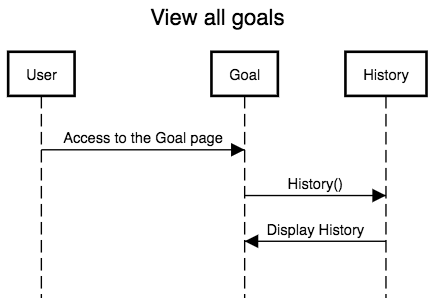
\includegraphics[width=\textwidth]{View_all_goals.png}
\newline
\newline
\newline
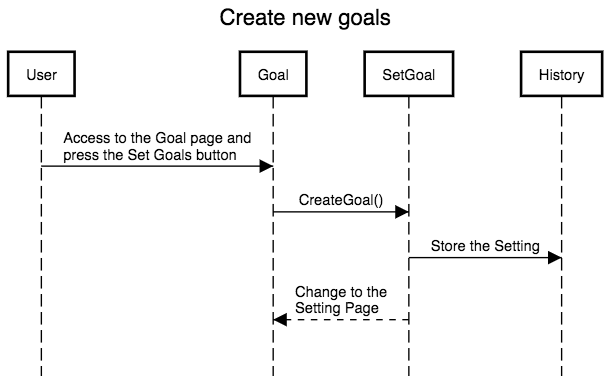
\includegraphics[width=\textwidth]{Create_new_goals.png}
\newline
\newline
\newline
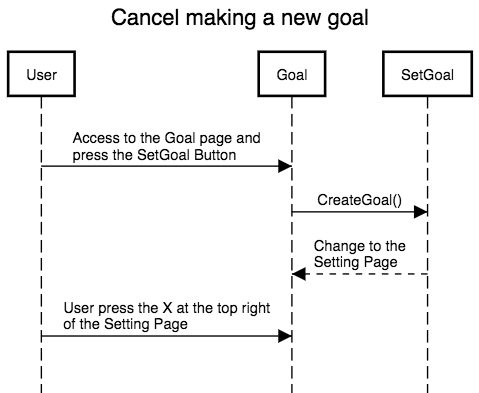
\includegraphics[width=\textwidth]{Cancel_making_a_new_goal.png}
\newline
\newline
\newline
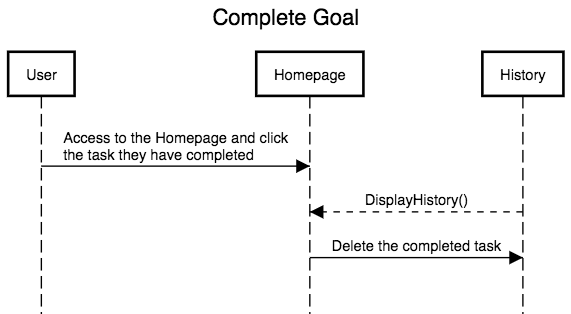
\includegraphics[width=\textwidth, height=8cm]{Complete_Goal.png}
\newline
\newline
\newline
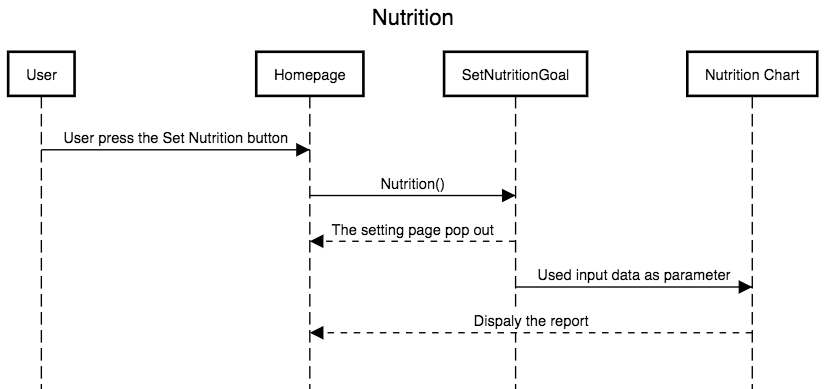
\includegraphics[width=\textwidth, height=8 cm]{Nutrition.png}
\newline
\newline
\newline
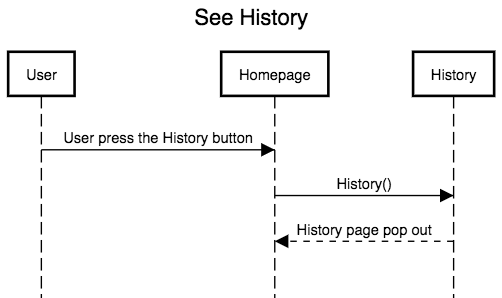
\includegraphics[width=\textwidth, height=8 cm]{See_History.png}
\newline
\section{The Stories due Next Week}

\subsection{View all goals}
We will have all the html/css skeleton framework in which the webpage will live implemented next week, then we will build the goal interface, that will show in a table the goals that the user had created.
\newline
\newline
Christa will implement the skeleton framework and the server that will support the project, Eric, Jorge, York and Blake will aid with the UI implementation.

\subsection{Create new goals}
For implementing the create new goal button, the user will click a button to create a goal then the user will be redirected to a page where we will make 2 menus, one that contain the possible goals to set (swim, lift, run, etc...) and other with an integer value that will be the distance, duration or number of sets for the selected goal.
\newline
\newline
Then the user will create the goal and this one will appear in a menu of all created goals that had not being completed yet.York, Christa, Eric and York will work in this part.

\subsection{Cancel making new goals}
We will add a cancel button to each created goals, so if the user decide to cancel a goal or if had made a mistake creating one, the goal can be eliminated. York, Christa and Blake will work in implement this feature.

\subsection{Complete goals}
If the user had completed the action of a previously created goal, he/she would be able to click a button that will mark the goal as completed, this action will make the goal disappear form the goals menu and allocate it into the history menu, when a goal is checked as completed, the system will award points to the user based in the goal numerical value(this feature will be implemented in other week). 
\newline
\newline
Next week Jorge, Eric and Christa will implement the completed goal feature, this feature will be partially completed because the points will not be awarded by the system, we expect to have completed the graphical indication that a goal has been completed and it redirection to the history menu.

\subsection{See History}
We will use nodejs to implement a database that will store the history of completed goals, the history will be displayed in its own menu for easy access by the user.
\newline
\newline
The history will show all the previously completed goals in a table, future releases will give the user the ability to re-do a previously completed goal form the history menu.
\newline
\newline
All the members of the team will brain storm in how to implement this feature, then Christa, Jorge, York will program it using nodejs, JavaScript other tools.



\section{Meeting Report}
This week we made a lot of progress! It was very productive in terms of working on code and project planning. We identified a few risks early on which involved the programmers to re-learn some of the programming languages we are using to develop our project. After some revision of old code and documentation provided on tutorial websites like w3schools.com and tutorialspoint.com/JavaScript, the programmers now have the knowledge and resources to work on several of our future planned spikes. 
\newline
\newline
Currently we have the HTML skeleton for our website. We are working on the user interface by styling the page using Bootstrap[6]. This being said we have about half of the front end part of our project developed. Some back-end has been created in the sense of developing a running server. No data has been allocated to be saved by user input yet. We will be using npm to install packets for our back-end server. 
\newline
\newline
So far each team member had made a effort to contribute to the projects. Christa has a lot of knowledge on web development, and has guided the group in what we need to learn and accomplish in order to have a working website. Eric and York have been designing the UML sequence diagrams for the tasks. Jorge and Blake have worked on documentation and planning. Each member has so far contributed coding. More coding is necessary in order for the project to be finished on time so all of us will be making an effort to contribute a lot more. 
\newline
\newline
The client was eager to meet with us. They were very interested in our product and its progress.We brain stormed about possible solutions and challenges related to the implementation of the webpage.Then we created a work plan, and delegate what features were feasible to be completed in this week and which would be able to be completed in future weeks.   
\newline
\newline
The tasks seemed difficult to accomplish at first. after running a few revisions on the tasks, we believe we will be able to accomplish them on time. We have spread the work out among the people involved in the project, so each person can contribute more equally.
\pagebreak
\section{Citations: }
[1] {https://www.railstutorial.org/book}\newline
[2]	{https://www.w3schools.com/}\newline 
[3] {https://github.com/}\newline
[4]{http://www.beyondorganic.net/dricalculator.html}\newline
[5] http://getbootstrap.com/\newline
[6]https://bootstrap.com/
\end{document}